\section{Сигмоидальный нейрон}

Для решения более сложных задач используются нейроны с непрерывными дифференцируемыми активационными функциями, которые не являются линейными. Один из таких нейронов – сигмоидальный нейрон.

Введение функций сигмоидального типа было обусловлено ограниченностью нейронных сетей с пороговой функцией активации нейронов — при такой функции активации любой из выходов сети равен либо нулю, либо единице, что ограничивает использование сетей в задачах, не связанных с классификацией. Использование сигмоидальных функций позволило перейти от бинарных выходов нейрона к непрерывным. Функции передачи такого типа, как правило, 
присущи нейронам, находящимся во внутренних слоях нейронной сети. \\

Сигмоидальный нейрон описывается математически следующим образом: \\

$
  f( \boldsymbol{x}, \boldsymbol{w}, b) = \sigma(\boldsymbol{wx} + b) \\
$

Где $ \mathlarger{\sigma(x) = \frac{1}{1 + e^{-x}}}$  - логистическая функция (Рис 1.3)

\begin{figure}[H]
  \centering
  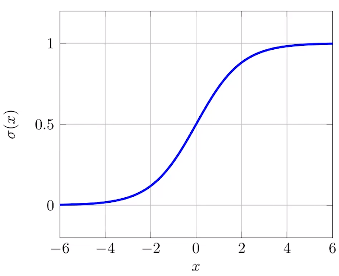
\includegraphics[width=0.5\linewidth]{./img/sigma-func}
  \caption{График логистической функции}
  \label{fig:mpr}
\end{figure} 

Особенностью нейронов с логистической функцией является то, что они усиливают сильные сигналы существенно меньше, чем слабые, поскольку области сильных сигналов соответствуют пологим участкам характеристики. Это позволяет предотвратить насыщение от больших сигналов.

Сигмовидные нейроны похожи на персептроны, но модифицированы так, что небольшие изменения их веса и смещения вызывают только небольшое изменение их выхода. Это решающий факт, который позволит сети сигмовидных нейронов учиться.


\subsection{Вывод правил обучения для логистического нейрона}
Используя данные полученные в главе 1.5.2, выведем правила обучения для сигмоидального нейрона.
Целевая функция остается такой же как и для линейного нейрона. Меняется только активационная функция, она будет иметь вид:

$$ \hat{y}^{(i)} = \sigma (w^T x^{(i)}) \eqno(10)$$

Следовательно меняется и частная производная:
$$
\frac{\partial J^{(i)}}{\partial w_j} = 
\frac{\partial J^{(i)}}{\partial \hat{y}^{(i)}} \cdot
\frac{\partial \hat{y}^{(i)}}{\partial S} \cdot
\frac{\partial S}{\partial w_j}
\eqno(11)
$$

Где $S = w^T x^{(i)}$ - сумматорная функция. Находим частные производные:

$$
\frac{\partial J^{(i)}}{\partial \hat{y}^{(i)}} = 
\sigma (w^T x^{(i)}) - y^{(i)}
\eqno(12)
$$

$$
\frac{\partial \hat{y}^{(i)}}{\partial S} = 
\frac{\partial \sigma (w^T x^{(i)})}{\partial (w^T x^{(i)})} =
\sigma (w^T x^{(i)}) \cdot (1 - \sigma (w^T x^{(i)}))
\eqno(13)
$$

$$
\frac{\partial S}{\partial w_j} = x_j^{(i)}
\eqno(14)
$$


Используя результаты (12), (13) и (14), находим градиент функции потерь:
$$
\nabla J = 
\frac{1}{n} \cdot \sum_{i=1}^{n}
\big(\sigma (w^T x^{(i)}) - y^{(i)}\big) \cdot
\sigma (w^T x^{(i)}) \cdot (1 - \sigma (w^T x^{(i)})) \cdot
x_j^{(i)}
\eqno(15)
$$
